\section{GPUE: GPU Gross--Pitaevskii equation solver}

As mentioned previously, the split operator method makes use of Fourier transforms as a way to change between position space and momentum space. To speed this up, the GPU accelerated CUFFT library is used, allowing for a much faster FFT than can be performed on a single (or across multiple) traditional CPU nodes. However, to take advantage of the GPUs performance, it is essential to minimise the data transfer between host machine (CPU) and device (GPU). Therefore, the remaining operations for the evolution must also be carried out on the GPU. This also requires that the workload is evenly distributed across the cores on the GPU so that we minimise the number of threads that are not performing computations.

Given that the problem of simulating the GPE in a rapidly rotating regime can be modeled as two-dimensional, we can put a limit on the


\begin{figure}
    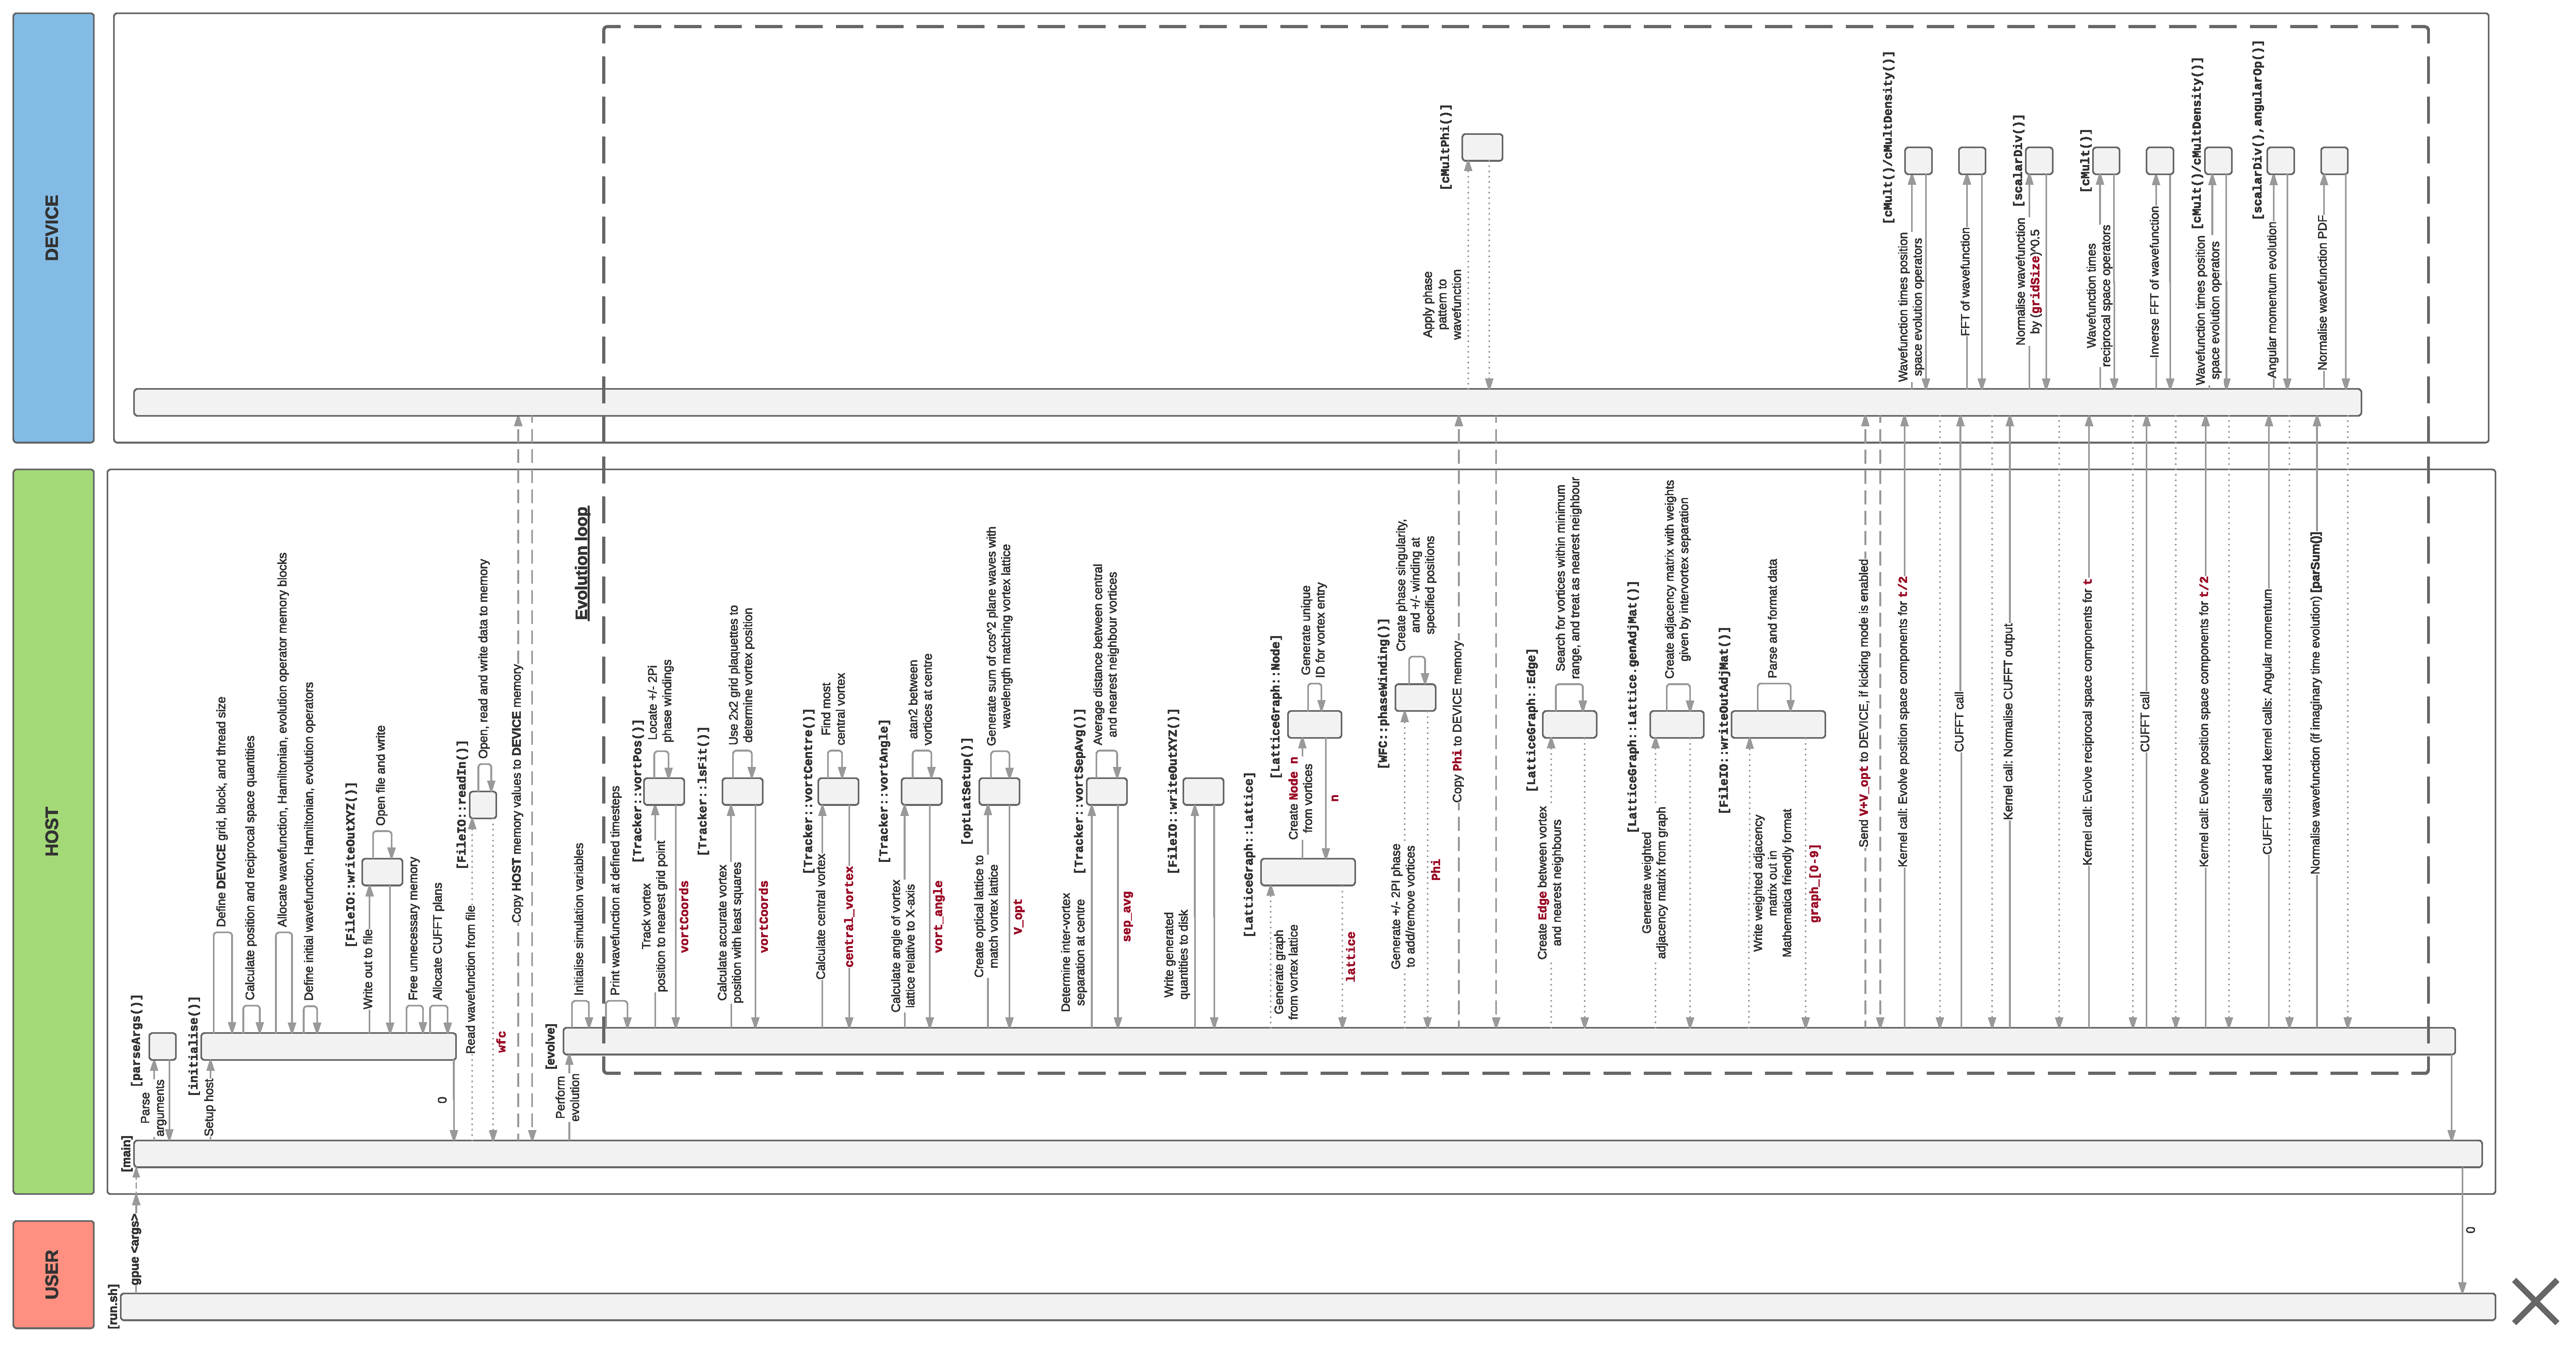
\includegraphics[width=1.5\textwidth,angle=270]{ch2_numerics/GPUE_Seq}
    \caption{Simplified combined sequence and state diagram for GPUE operation.}
    \label{fig:gpue_seq}
\end{figure}
